\chapter{Calibración utilizando acoplamientos mútuos}
\label{ch:convertidores}
\lhead{\emph{Calibración utilizando acoplamientos mutuos}}

\section{Calibración utilizando acoplamientos mutuos}

El método que utiliza los acoplamientos mutuos toma ventaja del acoplamiento mutuo inherente de un conjunto transmitiendo
y recibiendo entre elementos adyacentes. Para llevar a cabo dicho método, este tipo de antenas debe cumplir un
requerimiento muy importante que es poder transmitir con un elemento y simultáneamente recibir con otro sin que se sature o peor
aun, que se queme. Normalmente, este requerimiento implica separar las redes de transmisión y recepción \cite{Gao2001}. Para 
antenas que no cumplen la separación de la redes de transmisión y recepción se puede transmitir en una polarización y recibir
en otra. Por ende, es requisito para poder implementar el método que la red utilizada permita seleccionar los TRMs que van a 
estar en transmisión, en recepcion y en modo protegido. De esta forma, se establecen zonas en las cuales puede aplicarse el 
método actual dado que los niveles no son tan altos como para quemarlos ni tan bajos como para que no se alcance un nivel 
necesario para calibrar. La figura \ref{fig:levels} ejemplifica las tres zonas de recepción al emitir con un elemento radiante:
\begin{itemize}
	\item En rojo: zona de acoplamiento destructivo. Los TRMs deben estar protegidos.
	\item En verde: zona de acoplamiento dentro de los límites aceptables para aplicar el método.
	\item En azul: zona de acoplamiento débil. No se puede aplicar el método dado que el nivel de señal es inferior al piso de 
		ruido. 
\end{itemize}

\begin{figure}[H]
 \centering
 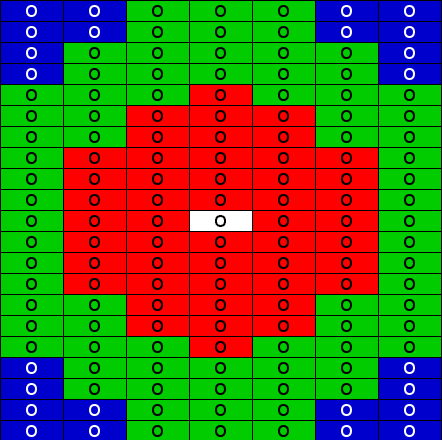
\includegraphics[width=9cm]{gfx/mutualCouplingLevels.png}
 \caption{Niveles de recepción de la antena al emitir con un elemento. En rojo, acoplamiento destructivo; en verde, 
 acoplamiento admisible y en azul acoplamiento débil.}
 \label{fig:levels}
\end{figure}

Para evitar que los elementos que no conforman parte del lazo activo de calibración interfieran, inyectando ruido en las redes 
de transmisión y/o recepción, se los debe poder configurar en modo alta impedancia (en este modo no se transmite ni recibe 
señal). En la figura \ref{fig:mutual_general} se puede observar un ejemplo.

\begin{figure}[H]
 \centering
 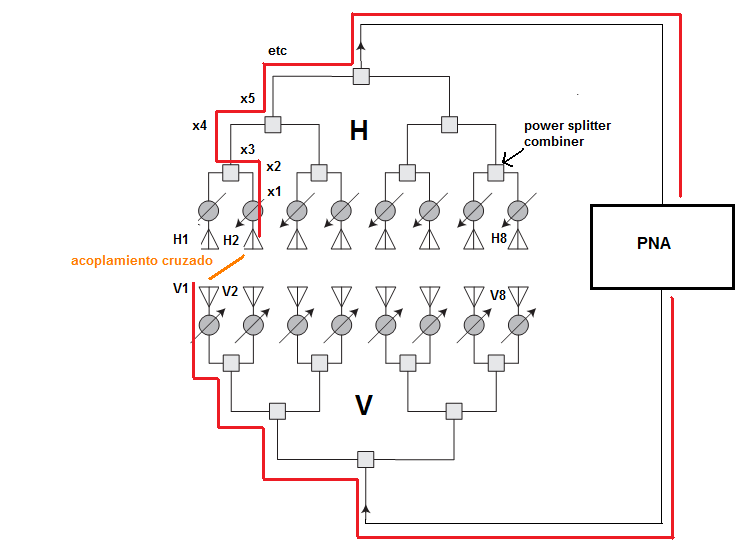
\includegraphics[width=9cm]{gfx/mutualCouplingExample.png}
 \caption{Ejemplo de calibración utilizando acoplamientos mutuos, transmitiendo en polarización V y recibiendo en H}
 \label{fig:mutual_general}
\end{figure}

En la figura \ref{fig:mutual_general} se puede observar un ejemplo en donde se transmite desde el elemento $e_1$ en 
polarización horizontal (H) y se recibe con el elemento $e_0$ en polarización vertical (V). Si se repite el proceso
secuencialmente con todos los elementos de recepción y luego con todos los elementos de transmisión, se puede determinar a
priori tanto la potencia de transmisión como la de recepción y lo que atenúa cada acoplamiento mutuo.

Como un primer paso, se determina que la cantidad de incógnitas que tiene una antena de $m$ elementos por $n$ paneles. Como
se puede transmitir y recibir en dos polarizaciones (H y V), la antena cuenta con $4MN$ incógnitas de RFDN (2 por Tx en H/V y
otras 2 por Rx en H/V). A su vez, en el apéndice \ref{AppendixA} se realiza el cálculo de la cantidad de acoplamientos mutuos
que posee una antena polarimétrica, particularmente, la ecuación \ref{eq:amountMutCoupling} muestra la cantidad de
incógnitas, que, para este caso, resulta ser de $MN(MN-1)/2$. Totalizando en $MN(MN + 7)/2$ incógnitas.

Asumiendo que se transmite de a un RM por lazo de calibración, a priori, se dispone de un máximo de $(MN)^2$ ecuaciones por
polarización a transmitir. Totalizando en $2(MN)^2$. Para que el sistema tenga solución, la cantidad de ecuaciones debe ser
mayor a la de las incógnitas, por lo tanto, la cantidad mínima de elementos radiantes es de

$$
\begin{aligned}
	2(MN)^2 &\ge  \dfrac{MN(MN + 7)}{2} \\
	4MN &- MN \ge7 \\
	MN &\ge \dfrac{7}{3}
\end{aligned}
$$

Como $M$ y $N$ son números enteros, con que la antena tenga tres o más elementos radiantes, ya se puede utilizar el método.

La herramienta matemática utilizada para resolver el sistema de ecuaciones es el de los cuadrados mínimos,
ver apéndice \ref{AppendixB}, con el cual se obtiene la aproximación que tenga menor error cuadrático medio.

Ante la posibilidad que no siempre se cuente con el tiempo necesario para generar todos los lazos de calibración necesarios
para calibrar la antena en el modo presentado, tres modalidades serán presentadas para este método.

\begin{itemize}
	\item \textbf{Modo completo:} En esta modalidad no solo se estima la ganancia en transmisión y recepción en ambas
		polarizaciones (H y V), sino que también se determinan los acoplamientos mutuos de la antena. La cantidad de ecuaciones necesarias es
		de $MN(MN + 7)/2$.
	\item \textbf{Modo rápido:} En esta modalidad se estima la ganancia en transmisión y recepción em ambas polarizaciones
		(H y V) utilizando el valor guardado de la planitud de la antena calculado previamente. La cantidad de ecuaciones necesarias
		es de $4MN$.
	\item \textbf{Modo planitud ideal:} Esta modalidad es igual al modo rápido, asuminedo que la antena es perfectamente plana.
		La cantidad de ecuaciones necesarias es de $4MN$.
\end{itemize}


\subsection{Método}

Asumiendo que se transmite desde el elemento $e_m$ y se recibe desde el $e_n$, la función de transferencia del lazo de
calibración está compuesta por:

\begin{itemize}
	\item La configuración de atenuación y defasaje de los defasadores y atenuadores, tanto de transmisión como de recepción,
		denotados como $w_{Tm}(i)$ y $w_{Rn}(j)$, donde $i$, $j$ son las diferentes posibles configuraciones.
	\item La atenuación y defasaje combinados por los cables, conectores, divisores y combinadores de potencia, módulos radiantes
		y defasadores, denotados como $u_{Tm}$ y $u_{Rn}$.
	\item El acoplamiento mutuo entre los elementos participantes, denotado como $C_{m, n}$.
\end{itemize}

Por lo tanto, la función de transferencia completa resulta,

\begin{equation}
	C^{'}_{m,n} = w_{Tm} u_{Tm} C_{m,n} w_{Rn} u_{Rn}
	\label{eq:transfer_mn}
\end{equation}

Si se transmite con el mismo elemento, $e_m$, pero se recibe con otro, $e_{n + 1}$, la transferencia resulta

\begin{equation}
	C^{'}_{m,n + 1} = w_{Tm} u_{Tm} C_{m,n + 1} w_{Rn + 1} u_{Rn + 1}
	\label{eq:transfer_mn1}
\end{equation}

Tomando la relación de ambas transferencias \ref{eq:transfer_mn} y \ref{eq:transfer_mn1},

\begin{equation}
	W^{m}_{Rn,n + 1} = \dfrac{C^{'}_{m,n}}{C^{'}_{m,n + 1}} = \dfrac{C_{m,n} w_{Rn} u_{Rn}}{C_{m,n + 1} w_{Rn + 1} u_{Rn + 1}}
\end{equation}

Se asume que el valor del acoplamiento depende de dos factores a saber. El primero es por comunicar los elementos utilizando
polarizaciones cruzadas, y dicha atenuación es constante para cualquier elemento. El segundo, es debido a la atenuación y
defasaje de la señal que viaja en el vacío, por lo tanto, depende exclusivamente de la distancia que hay entre los elementos
a comunicar.

Ahora, si se combinan las funciones de transferencia $C^{'}_{m,n+1}$ y $C^{'}_{m,n+2}$, la relación resulta,

\begin{equation}
	W^{m}_{Rn + 1,n + 2} = \dfrac{C^{'}_{m,n+1}}{C^{'}_{m,n+2}} = \dfrac{C_{m,n+1} w_{Rn+1} u_{Rn+1}}{C_{m,n + 2} w_{Rn + 2} u_{Rn + 2}}
\end{equation}

Ahora, si se combinan las funciones de transferencia $C^{'}_{m,n}$ y $C^{'}_{m,n+2}$,

\begin{equation}
	W^{m}_{Rn,n + 2} = \dfrac{C^{'}_{m,n}}{C^{'}_{m,n + 2}}\cdot\dfrac{C^{'}_{m,n+1}}{C^{'}_{m,n+1}} = W^{m}_{Rn,n+1}\cdot W^{m}_{Rn+1,n + 2}
\end{equation}

Generalizando, se pueden obtener todos los lazos de calibración en función de uno,

\begin{equation}
	W^{m}_{R0,k} = \prod_{i=0}^{k-1} W^{m}_{Ri,i+1} = \prod_{i=0}^{k-1}\dfrac{C^{'}_{m,i}}{C^{'}_{m,i+1}} =
		\prod_{i=0}^{k-1}\dfrac{C_{m,i} w_{Ri} u_{Ri}}{C_{m,i + 1} w_{Ri + 1} u_{Ri + 1}}
	\label{eq:rx_cal}
\end{equation}

Si se realiza la misma deducción, pero en vez de transmitir siempre con el mismo elemento, se lo utiliza para recibir, se obtiene

\begin{equation}
	W^{m}_{T0,k} = \prod_{i=0}^{k-1} W^{m}_{Ti,i+1} = \prod_{i=0}^{k-1}\dfrac{C^{'}_{i,m}}{C^{'}_{i+1, m}} =
		\prod_{i=0}^{k-1}\dfrac{w_{Ti} u_{Ti} C_{i,m}}{w_{Ti + 1} u_{Ti + 1}C_{i + 1, m}}
	\label{eq:tx_cal}
\end{equation}

Analizando las ecuaciones \ref{eq:rx_cal} y \ref{eq:tx_cal}, dos conclusiones inmediatas se deducen. La primera es que el
resultado no es único, por lo tanto, en principio, con este método no se pueden obtener ganancias absolutas (de transmisión,
recepción y acoplamientos mútuos), solamente ganancias relativa entre dichos elementos. La segunda, es que el sistema tiene
dos grados de libertad, en otras palabras, para poder obtener la ganancia absoluta de todo el sistema, es necesario agregar
dos ecuaciones más que definan algún valor pertenenciente a dos de los tres conjuntos de incógnitas.

Si se asume que a misma distancia el acoplamiento es el mismo o si se los reutilizan de una calibración anterior, las
ecuaciones \ref{eq:rx_cal} y \ref{eq:tx_cal} se simplifican, logrando que la cantidad de incógnitas se reduzca habilitando
de esta forma los métodos rápidos y de planitud ideal. 

Como es necesaria una menor cantidad de ecuaciones de calibración, la estrategia a encarar es la de utilizar lazos simétricos
con un elemento en común. Al restar ambos caminos, no solo se elimina la RFDN común, sino que también se elimina el
acoplamiento mútuo. La cantidad de estos lazos termina siendo determinada como una solución de compromiso entre la cantidad de
mínima necesaria para poder utilizar el método y la cantidad de ecuaciones redundantes para disminuir la incertidumbre en el
resultado. Las ecuaciones para recepción y transmisión simplificadas resultan.

\begin{equation}
	W^{'}_{R0,k} = \prod_{i=0}^{k-1} W^{'}_{Ri,i+1} = \prod_{i=0}^{k-1}\dfrac{w_{Ri} u_{Ri}}{w_{Ri + 1} u_{Ri + 1}} =
	\dfrac{w_{R0} u_{R0}}{w_{Rk} u_{Rk}}
	\label{eq:rx_simp_cal}
\end{equation}

\begin{equation}
	W^{'}_{T0,k} = \prod_{i=0}^{k-1} W^{'}_{Ti,i+1} = \prod_{i=0}^{k-1}\dfrac{w_{Ti} u_{Ti}}{w_{Ti + 1} u_{Ti + 1}} =
	\dfrac{w_{T0} u_{T0}}{w_{Tk} u_{Tk}}
	\label{eq:tx_simp_cal}
\end{equation}

Si el RM común se utiliza para transmitir la señal, se obtienen ecuaciones para calibrar la parte de recepción, en cambio,
si se lo utiliza para recibir la señal, se calibra transmisión. La figura \ref{fig:ideal_strategy} esquematiza esta estrategia.

\begin{figure}[H]
 \centering
	\subfloat[]{
		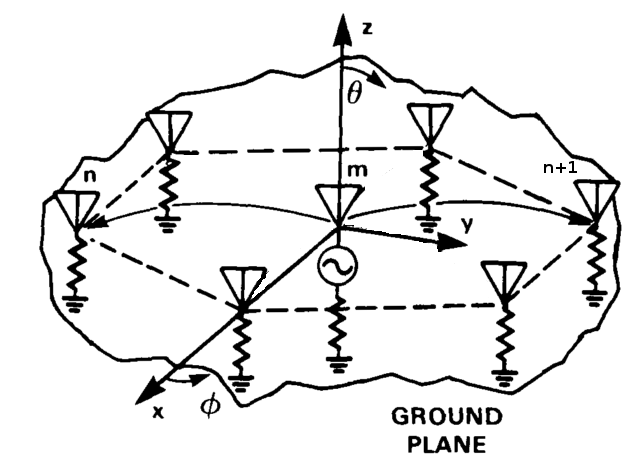
\includegraphics[width=5cm]{gfx/mutualRxCal.png}}
	\subfloat[]{
		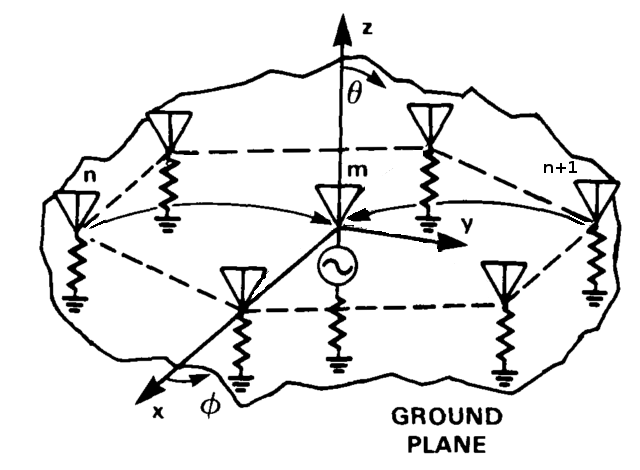
\includegraphics[width=5cm]{gfx/mutualTxCal.png}}
	\caption{estrategia de planitud ideal. (a) Calibra lazos de recepción, (b) Calibra lazos de transmisión \cite{Aumann1989}.}
 \label{fig:ideal_strategy}
\end{figure}

\subsection{Determinación de la fase} \label{ssc:mutualPhase}

Como el método de resolución utilizado en este método es de naturaleza lineal, resolviendo ecuaciones del estilo $Ax = b$, y
como la fase de una señal es de naturaleza modular, de 360 grados, se pueden cometer errores en la resolución. Dependiendo de
como sea $A$ y que valores tenga $x$, $b$ no necesariamente está contenido dentro del conjunto solución (en módulo 360)
generando así un error en la resolución de la estimación del valor $x$.

Para ejemplificar, se asume que se tiene un conjunto de antena de tres elementos radiantes. La RFDN (en Tx y Rx) defasa 100
grados, el defasador del primer elemento está configurado en 240 grados y el del tercero en 120, el acoplamiento mutuo no defasa
y se utiliza la ecuación $\dfrac{C^{'}_{1,2}}{C^{'}_{3, 2}}$. La figura \ref{fig:phaseDetermination} muestra la antena con los 
lazos de calibración utilizados.

\begin{figure}[H]
 \centering
 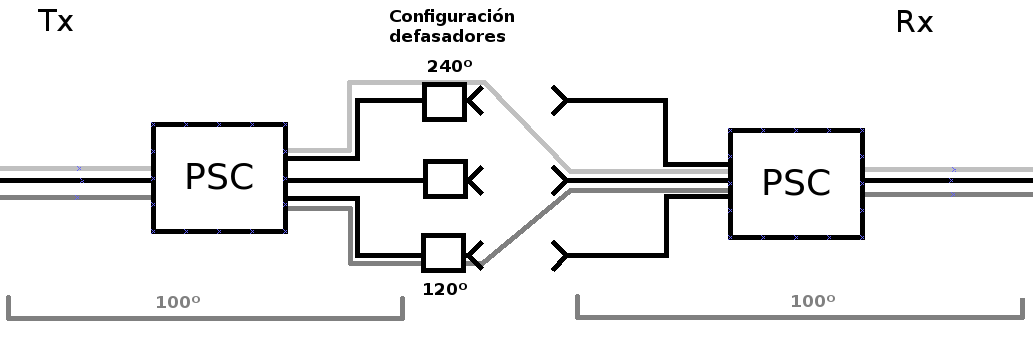
\includegraphics[width=10cm]{gfx/loopCal.png}
 \caption{Lazo de calibración de una antena polarimétrica}
 \label{fig:phaseDetermination}
\end{figure}

Utilizando la ecuación previamente mencionada, $A$ resulta ser
$$
	\mathbf{A} = \begin{pmatrix} 1 & 0 & -1\end{pmatrix}
$$
El verdadero valor de x resulta ser la contribución de la rama de transmisión junto a la configuración del defasador del TRM,
$$
	\mathbf{x} = \begin{pmatrix} 340 \\ x \\ 220\end{pmatrix}
$$

Al resolver la ecuación $Ax$ se obtiene el resultado de 120 grados. Si la fase fuese de naturaleza lineal, este sería el valor 
resultante de la resta de la medición de ambos lazos de calibración. Las mediciones de dichos lazos resultan: 
\begin{itemize}
	\item La fase de $C^{'}_{1,2}$ es 440 grados, en módulo 360 resulta igual a 80 grados (100 grados por la rama de
		transmisión sumado a 240 por el defasador del primer TRM y 100 grados más por la rama de recepción).
	\item La fase de $C^{'}_{3, 2}$ es 320 grados (100 grados por la rama de transmisión sumado a 240 por el defasador
		del primer TRM y 100 grados más por la rama de recepción).
\end{itemize}

La resta de dichas mediciones deberían ser igual a 120 grados, pero se observa que es igual a -240 grados generando así un
error en la estimación de la fase.

Para soluciona esto, la estrategia propuesta es la de reutilizar el valor estimado de $x$ de una calibración previa, calcular
el $b$ ideal y modificar los valores de $b$ de la calibración actual sumando o restando de a 360 grados para acercarse lo más 
posible a dichos valores esperados. Para la primera calibración, es necesario medir cuanto defasa la antena en al menos una 
rama punta a punta. 

\subsection{Problemas y limitaciones}

La mayor limitación de este método es que es necesario conocer, a groso modo, el valor del defasaje de uno de los caminos de
Tx o Rx punta a punta. Esto es para poder evitar errores de cálculos al obtener la fase de transmisión o recepción del
sistema, ya que la misma tiene un comportamiento modular. Dicho valor solo se lo utilizará una vez, dado que ya para las
subsiguientes calibraciones, el valor previo de fase de la antena es conocido y reutilizado. 

Para obtener dicho valor inicial, se puede utilizar la fase delvuelta por el método de calibración clásica o se puede realizar
una medición de campo cercano en temperatura, emitiendo sólamente con un elemento radiante para deducir la fase de la red de 
transmisión, para obtener el defasaje de la red de recepción, se emite con un elemento externo y se recibe con solo un elemento
radiante. 
